\appendix
\chapter{Python skript pro symbolické určení nejistot přísunů radonu}\label{navesti:priloha_nejistoty}
\lstinputlisting[language=Python]{nejistoty.py}

\chapter{Python skript pro vyhodnocení dynamického měření přísunů radonu}\label{navesti:priloha_dynamickeMereni}

\chapter{Přílohy k objektu Skála 75, okr. Havlíčkův Brod}
\section{Schéma objektu}\label{navesti:priloha_skala75}

\section{Naměřené vývoje OAR, teplot a relativní vlhkosti vzduchu}
\begin{figure}[H]
    \centering
    %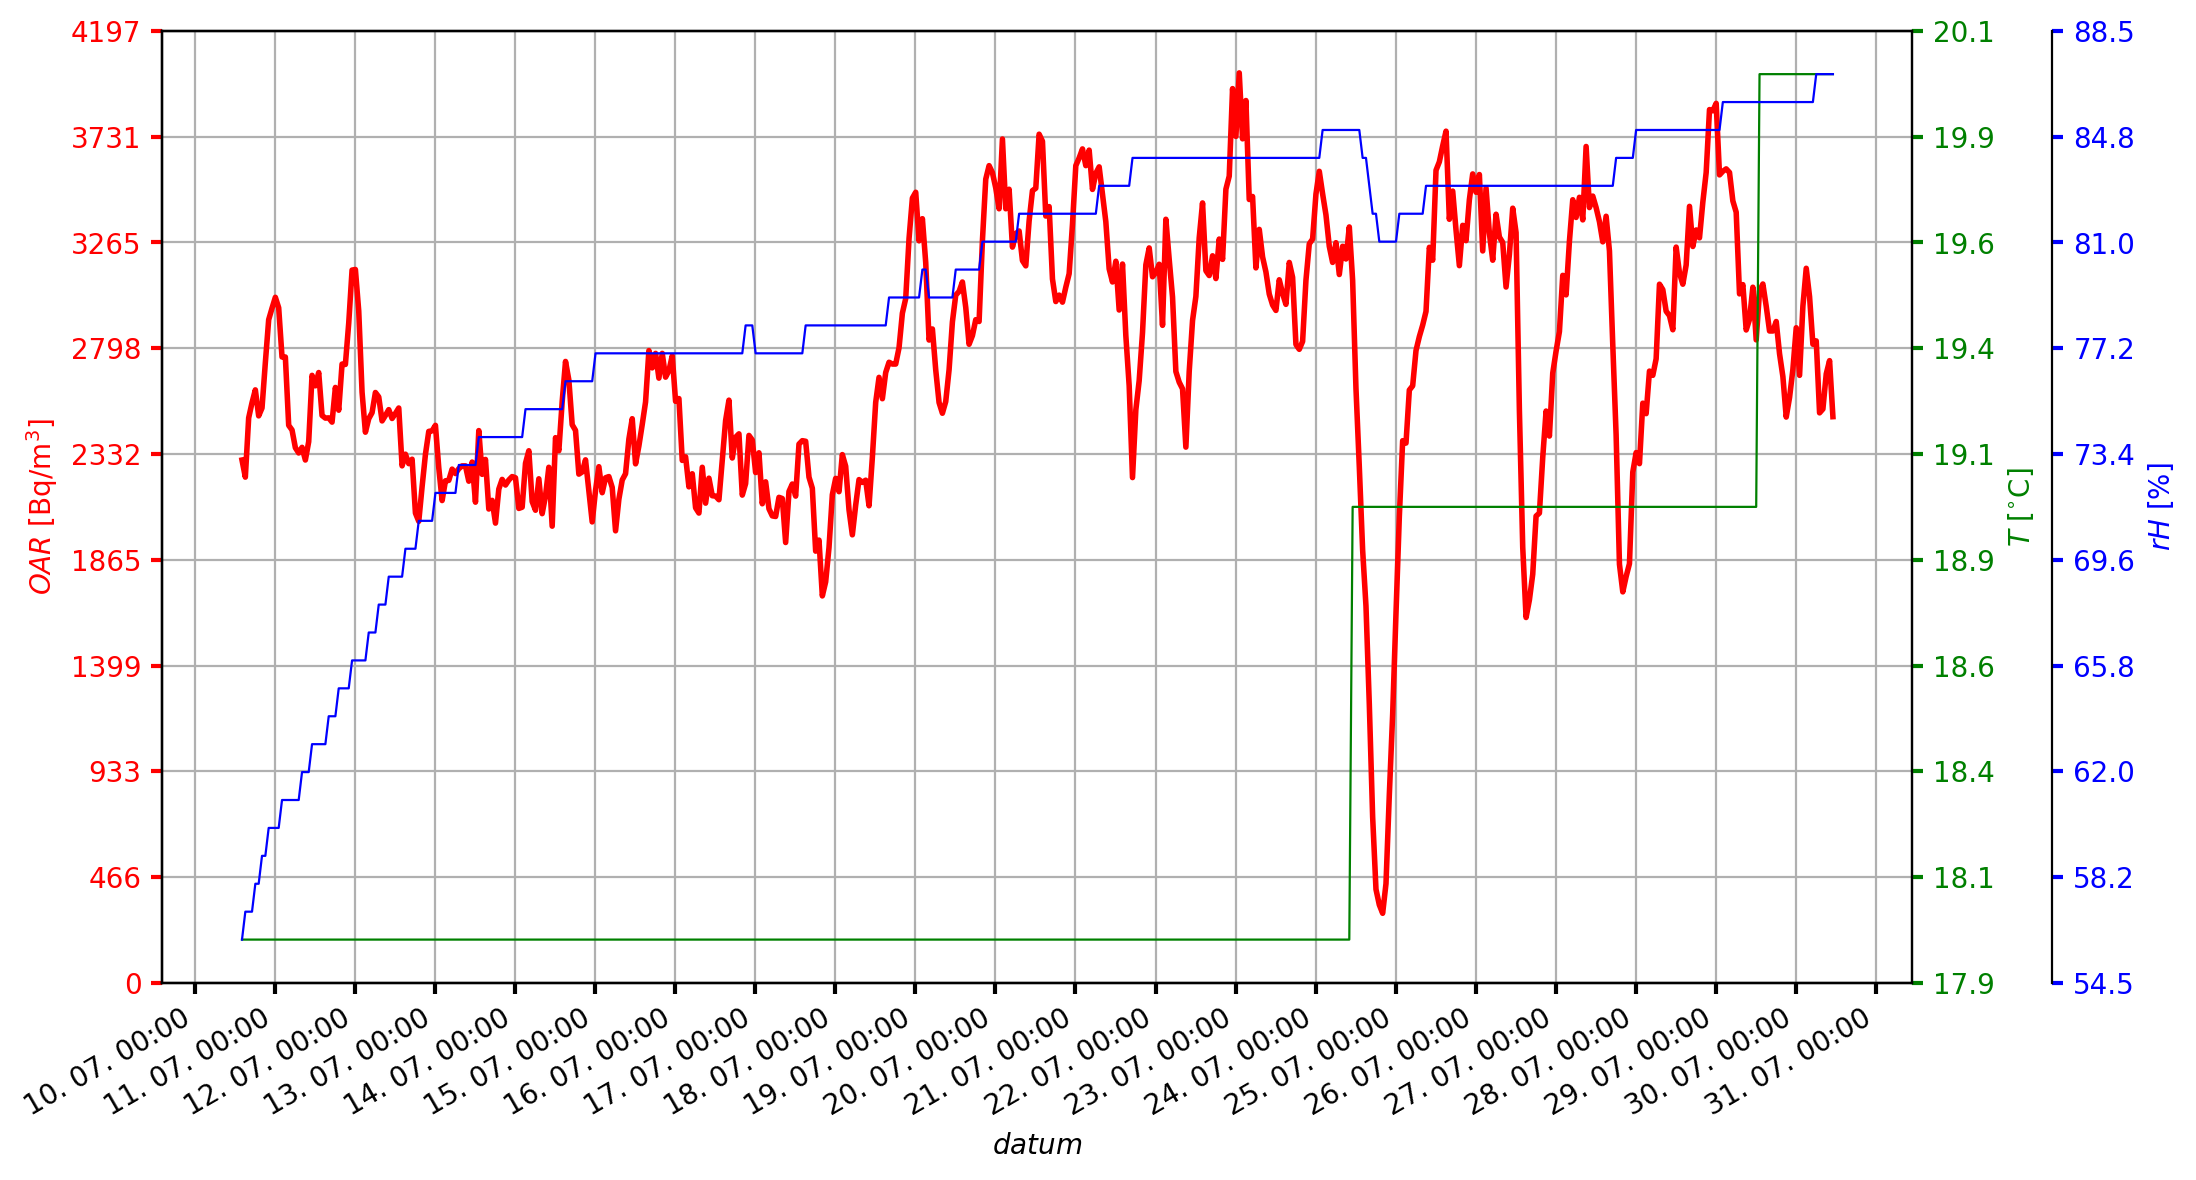
\includegraphics[height=0.8\textwidth, angle=-90, origin=c]{skala75/a1.png}
    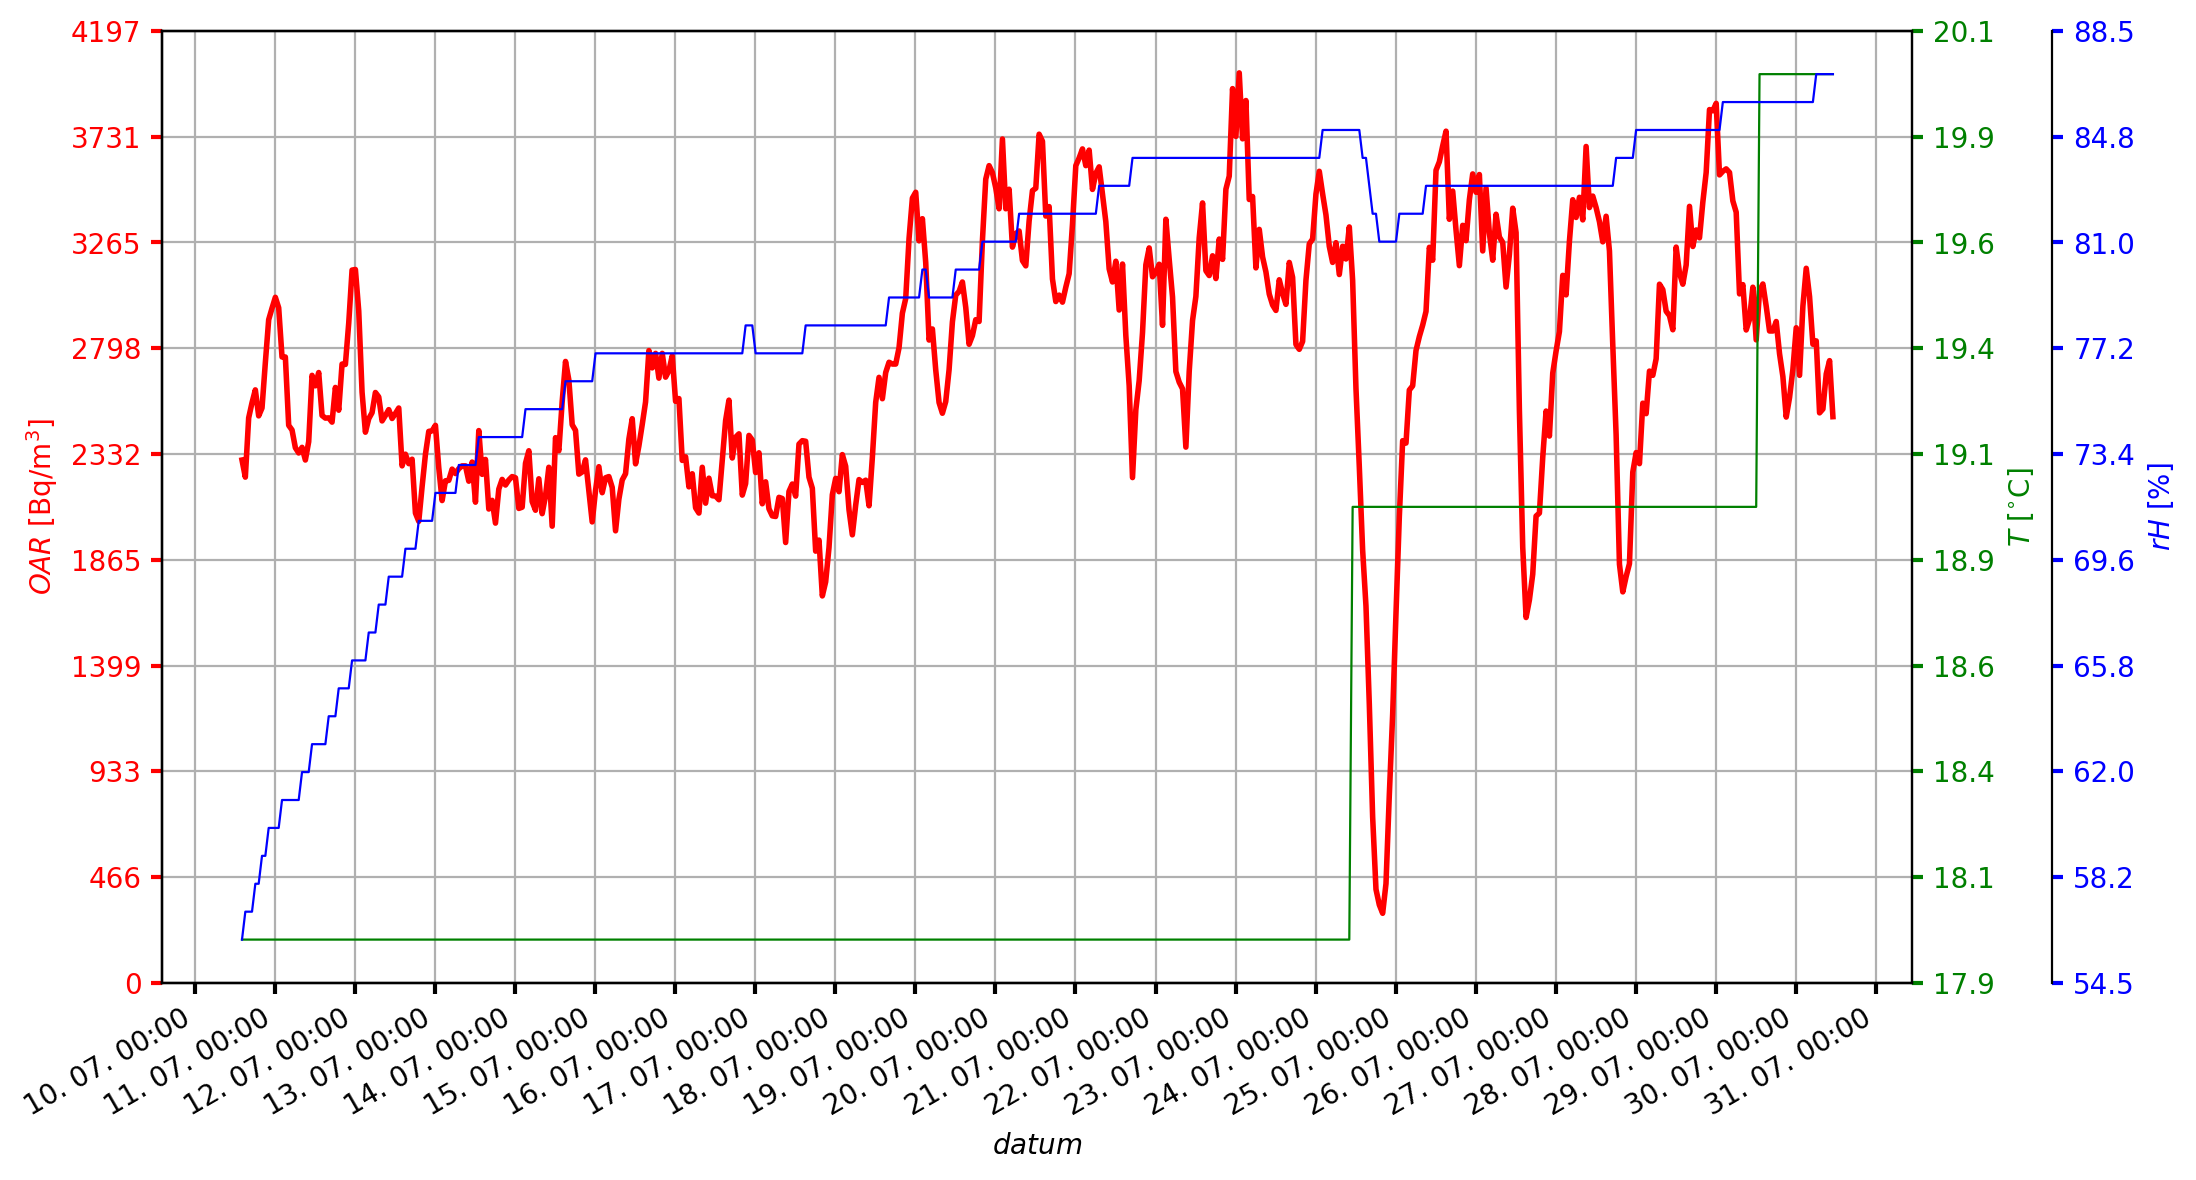
\includegraphics[width=1.1\textwidth]{skala75/a1.png}
    \caption{Data z TERA sondy č. 8, která byla umístěna ve sklepě.}
    \label{fig:skala75_a1}
\end{figure}
\begin{figure}[H]
    \centering
    %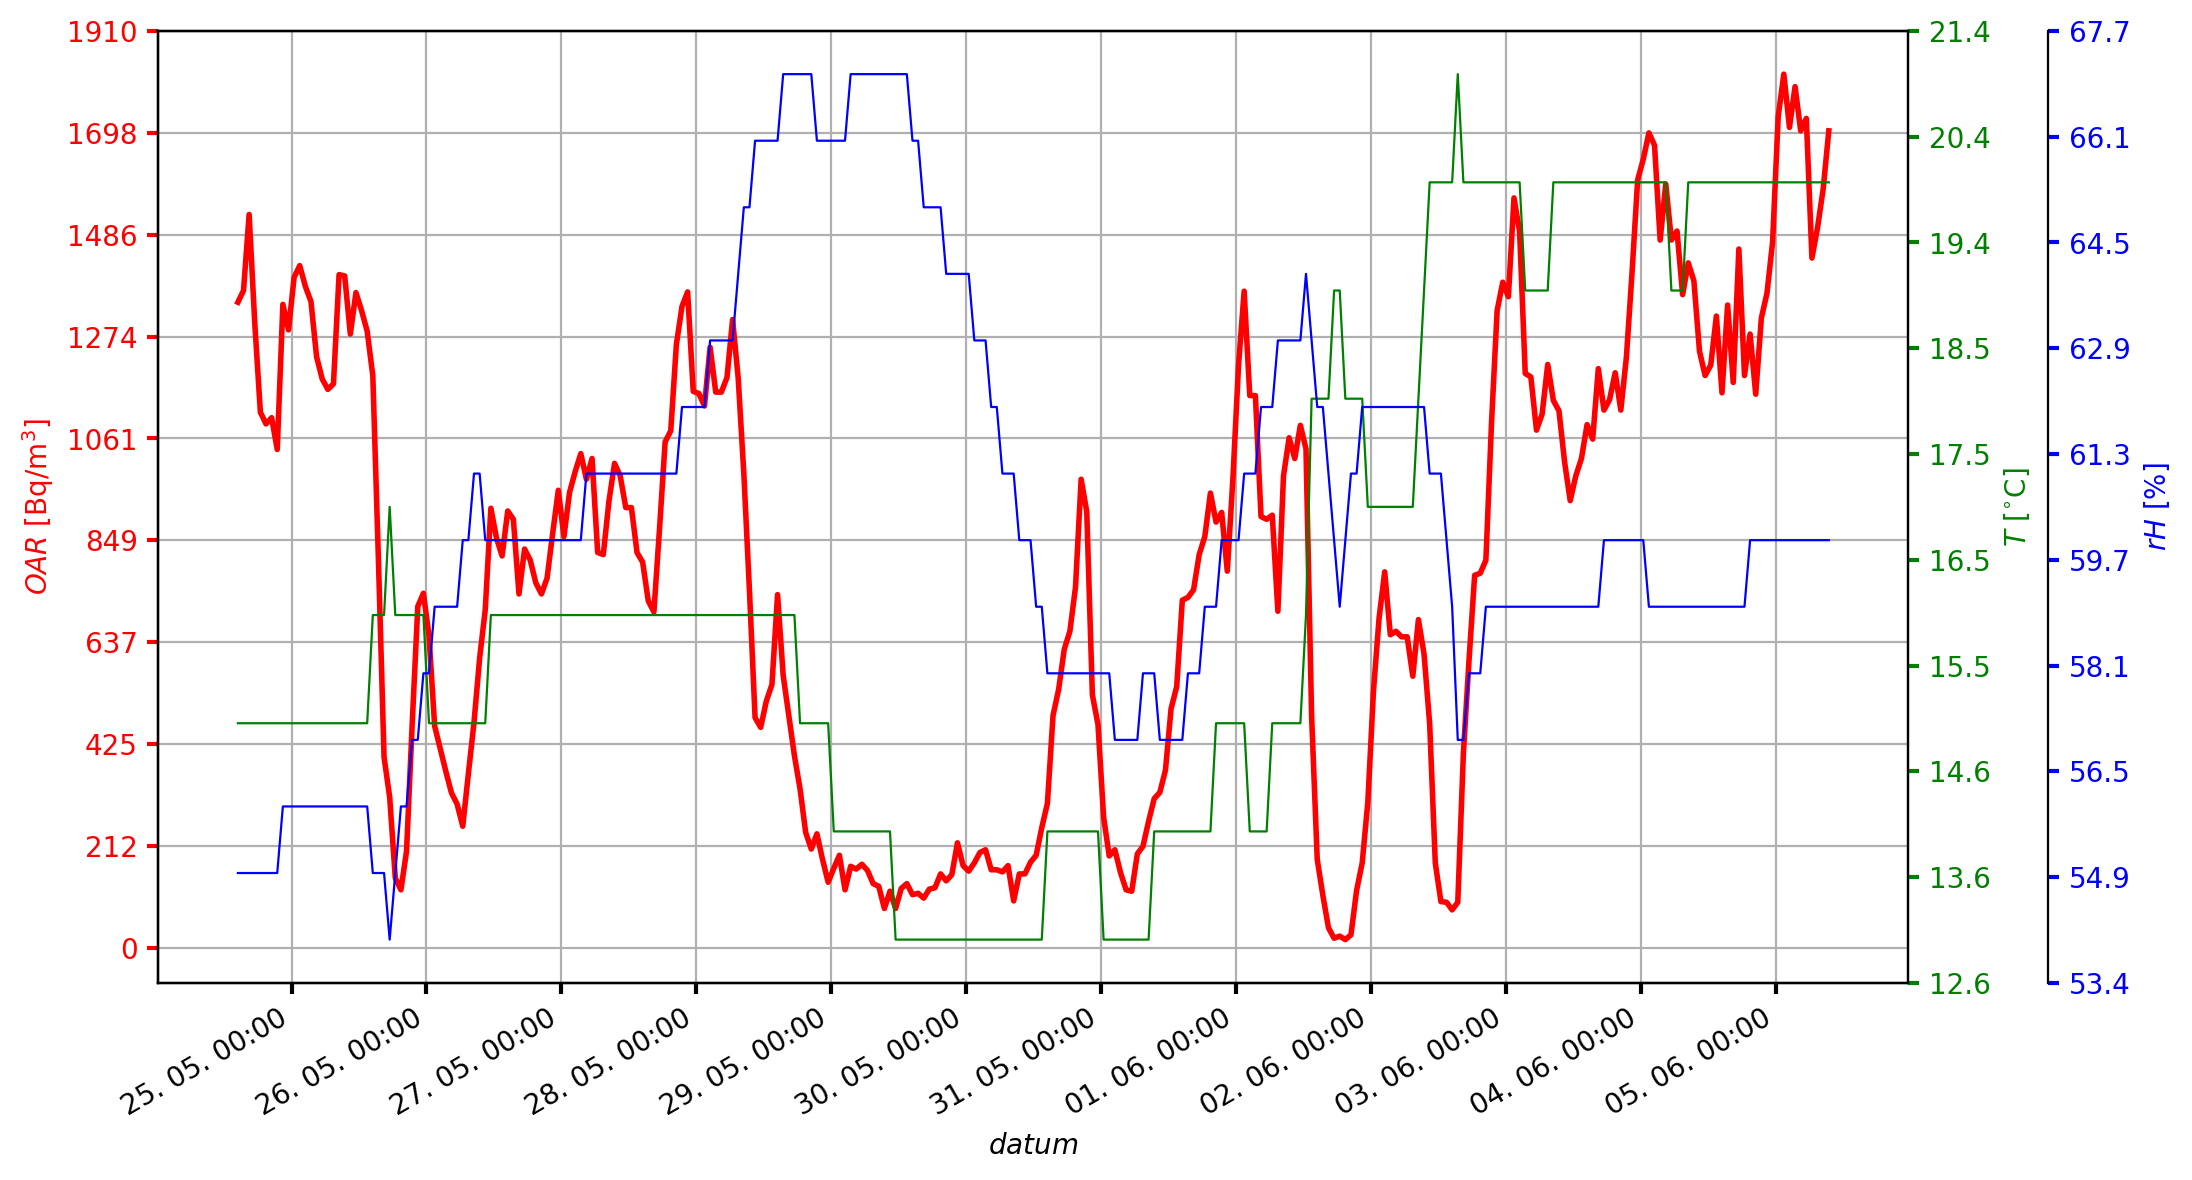
\includegraphics[height=0.8\textwidth, angle=-90, origin=c]{skala75/a2_1.png}
    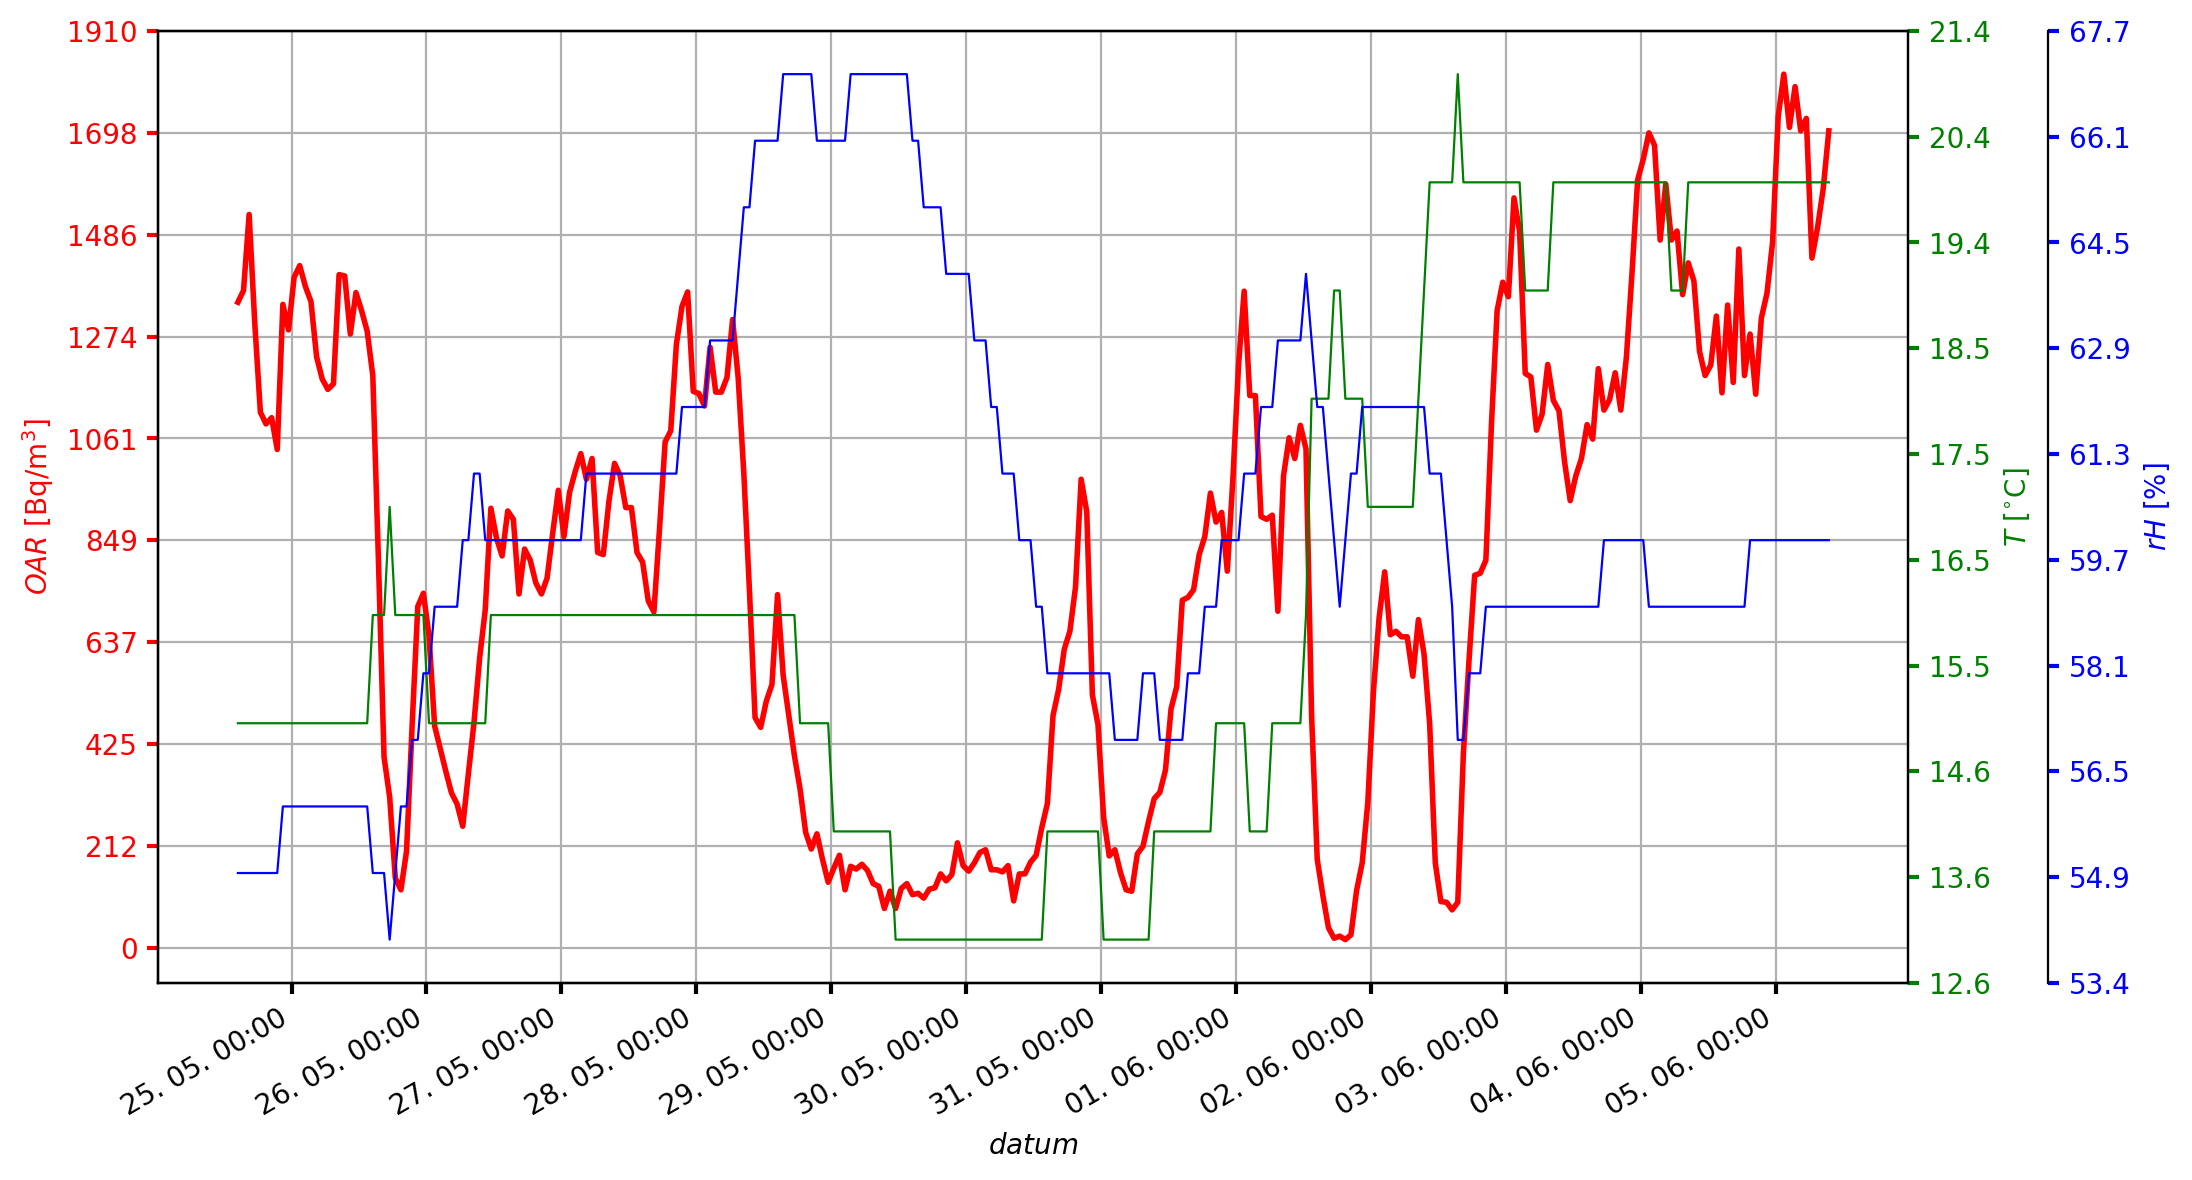
\includegraphics[width=1.1\textwidth]{skala75/a2_1.png}
    \caption{Data z TERA sondy č. 10, která byla umístěna v přízemí v kuchyni.}
    \label{fig:skala75_a2_1}
\end{figure}
\begin{figure}[H]
    \centering
    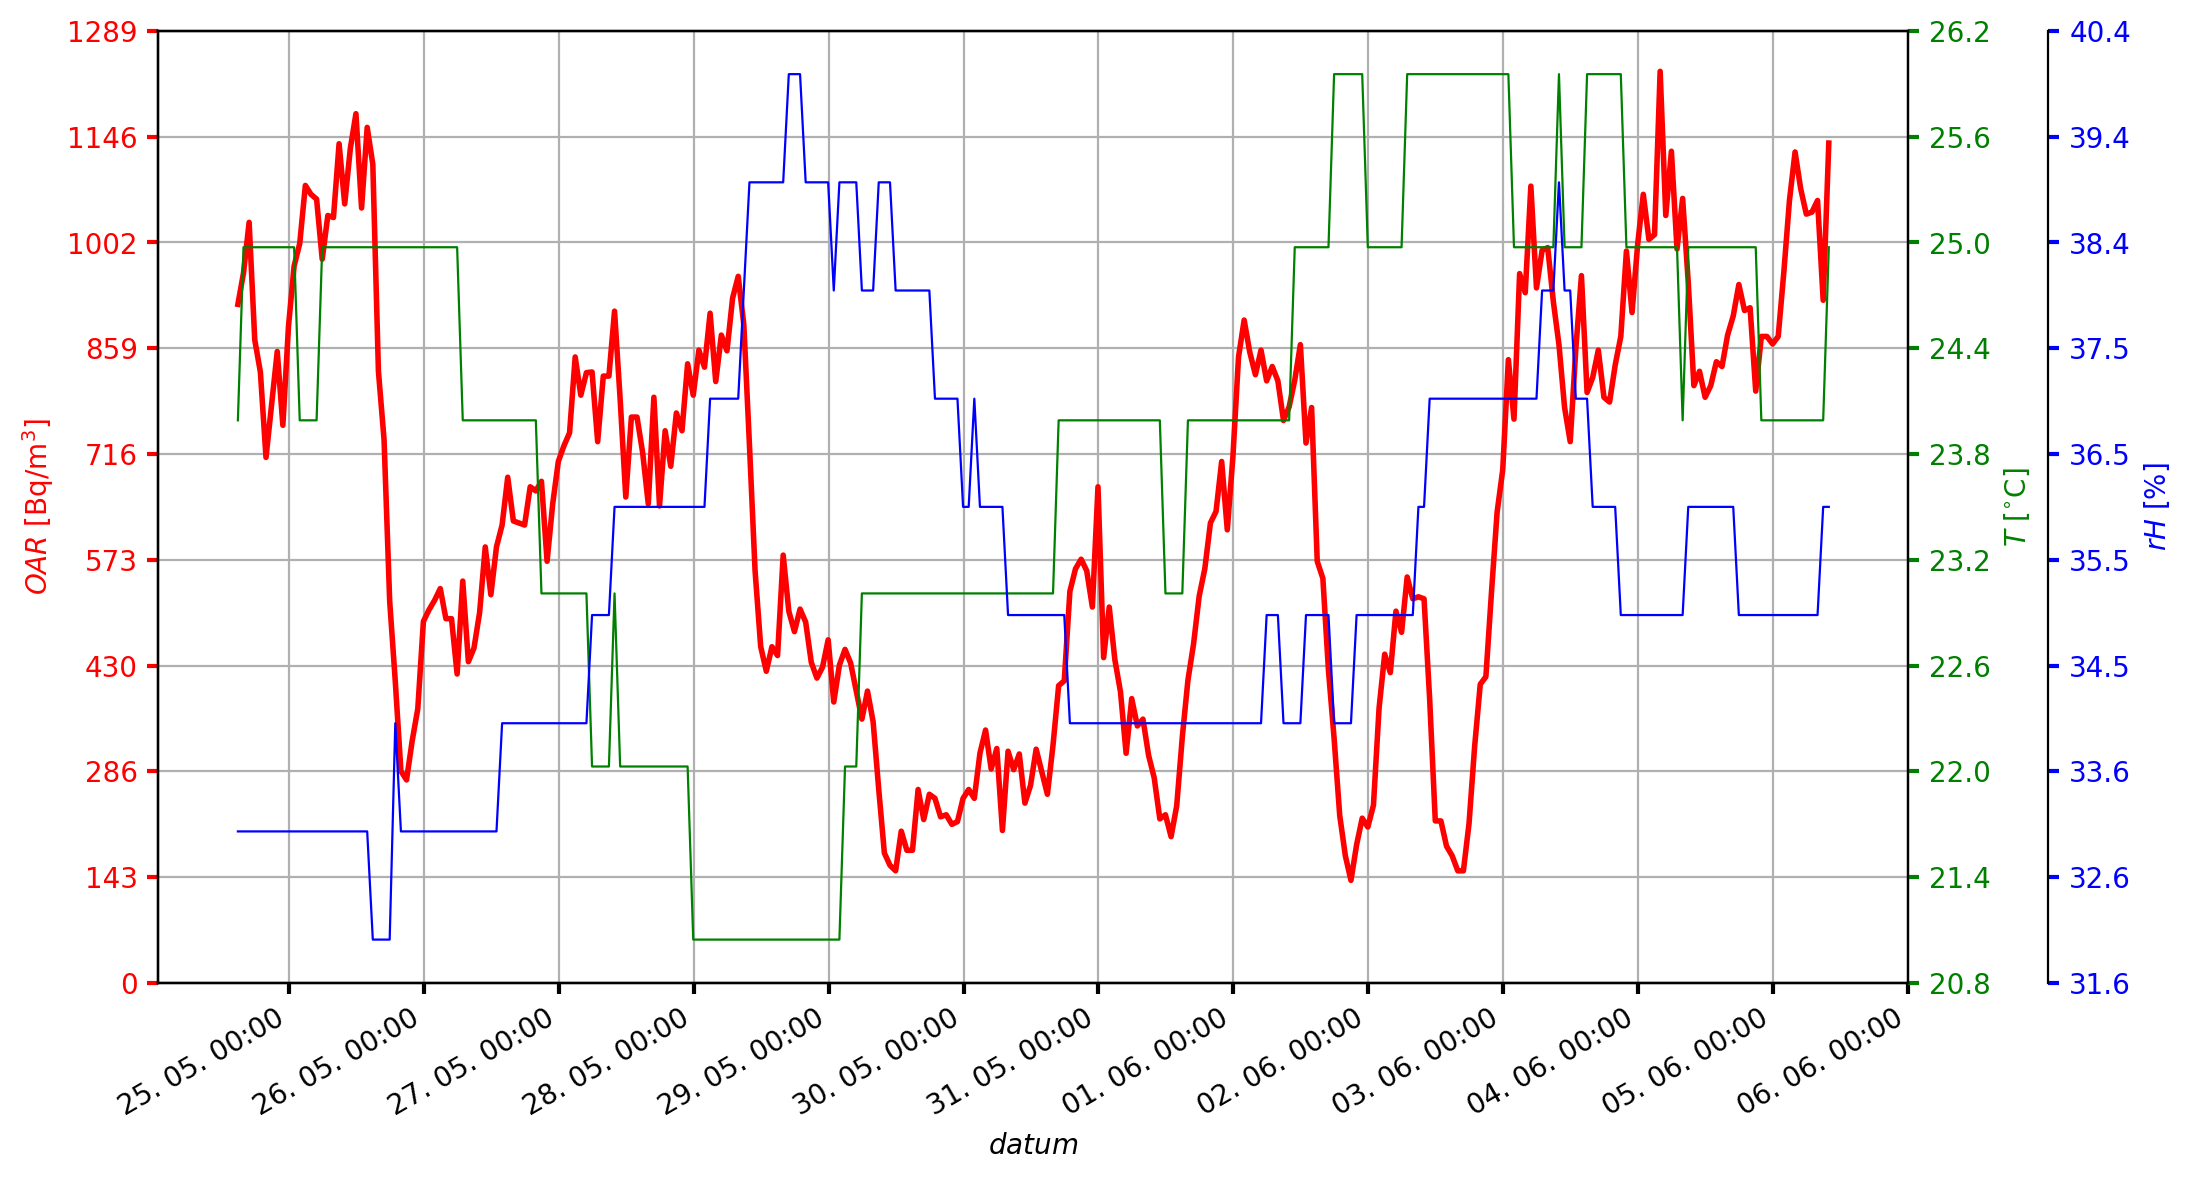
\includegraphics[width=1.1\textwidth]{skala75/a2_2.png}
    \caption{Data z TERA sondy č. 112, která byla umístěna v přízemí v ložnici.}
    \label{fig:skala75_a2_2}
\end{figure}
\begin{figure}[H]
    \centering
    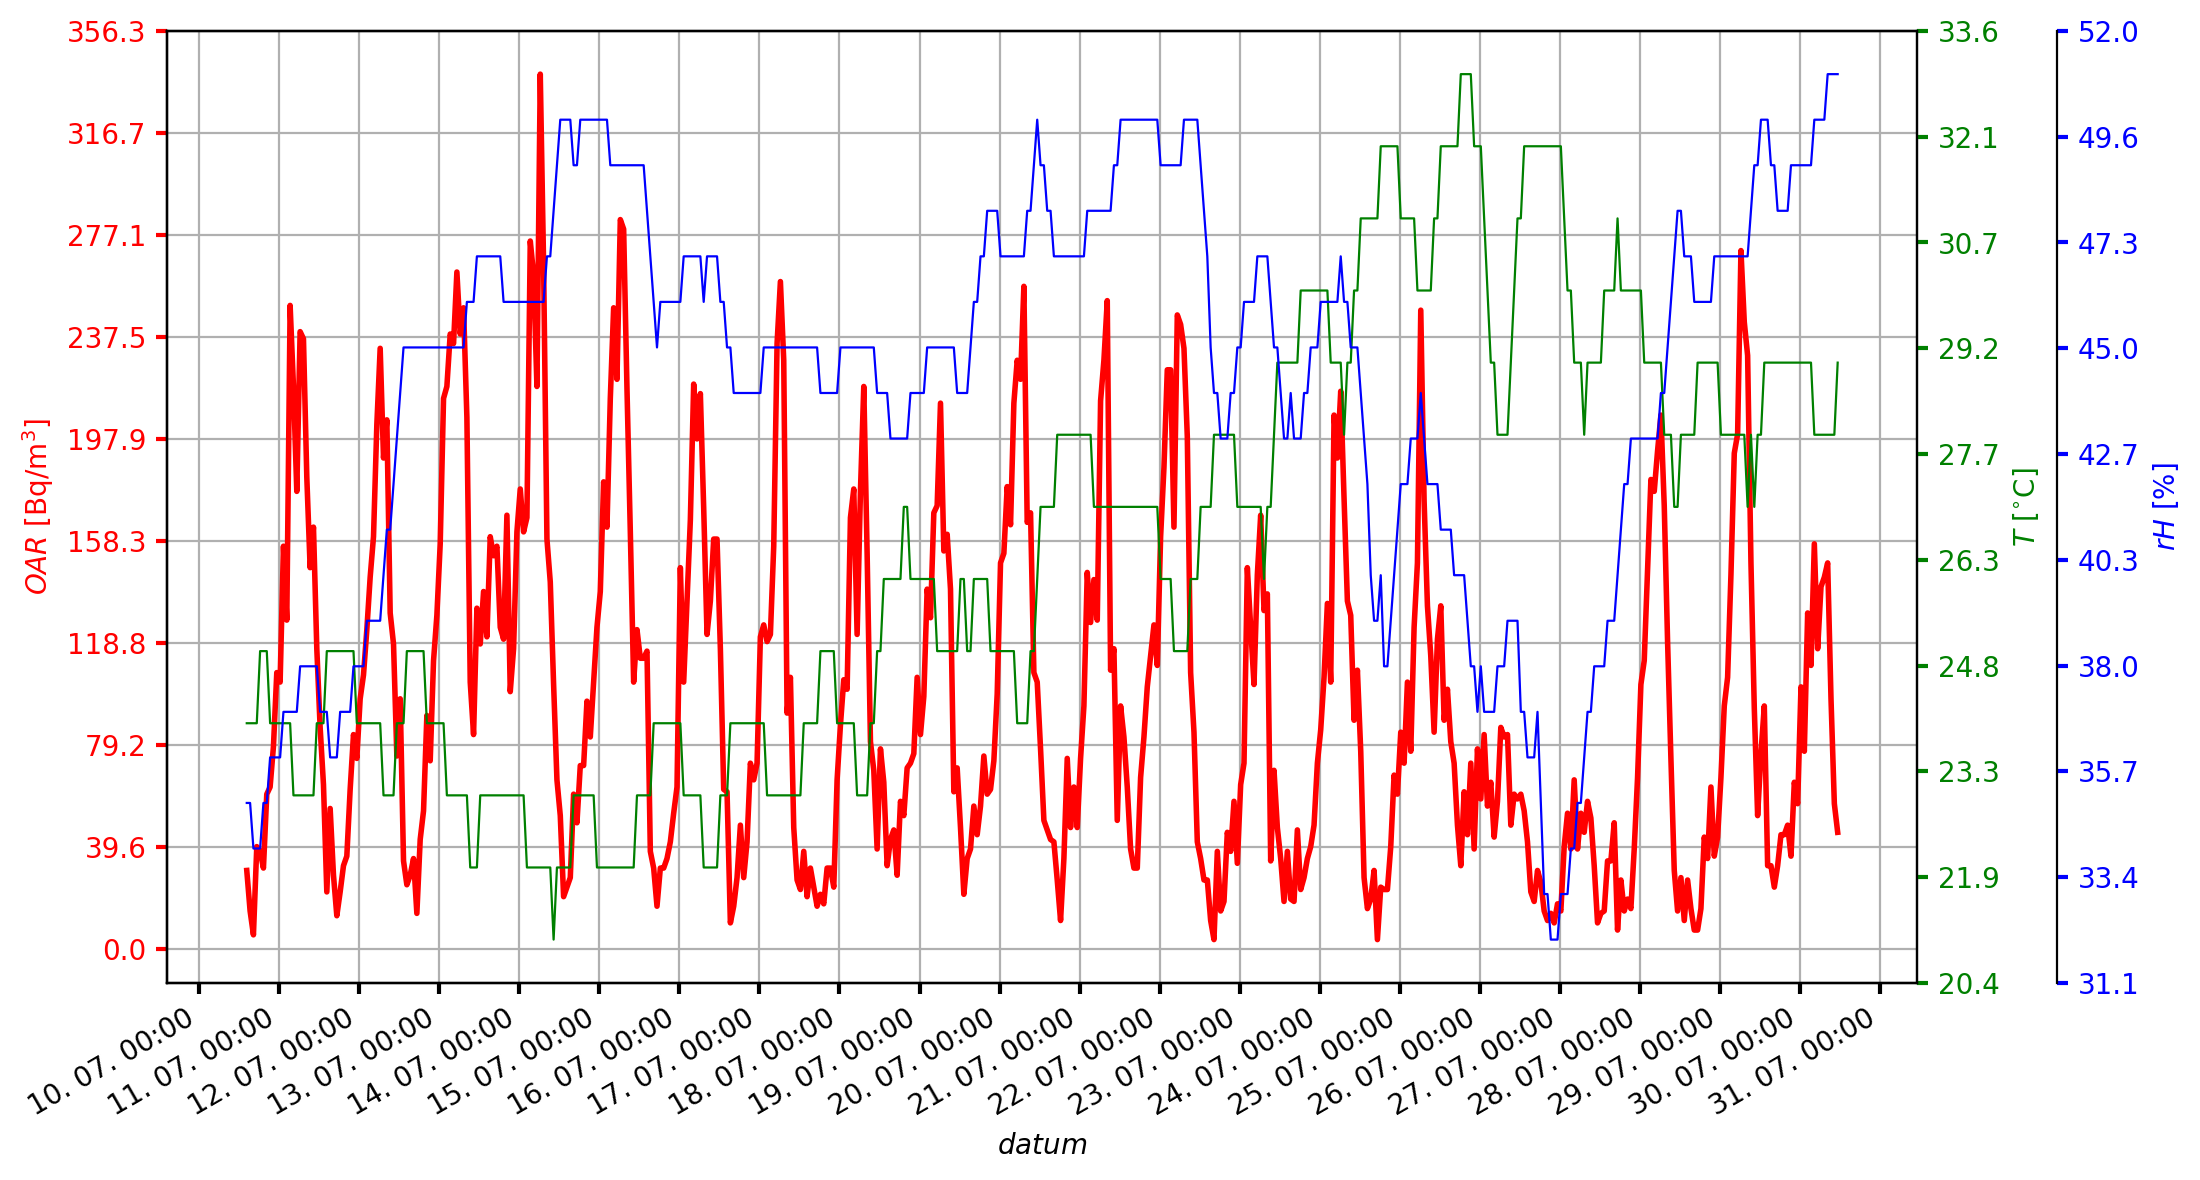
\includegraphics[width=1.1\textwidth]{skala75/a3.png}
    \caption{Data z TERA sondy č. 88, která byla umístěna v prvním patře.}
    \label{fig:skala75_a3}
\end{figure}

